\chapter*{Antarctica's Landscape}\label{why}
\section*{Climate Impacts and Global Significance}

The polar regions are losing ice, and their oceans are changing rapidly\cite{O_C_in_changingClimate}. The consequences of this polar transition extend to the whole planet and it is crucial for us to understand them, to be able to evaluate the costs and benefits of potential mitigation strategies. 

The consequences of changes in different kinds of polar ice manifest across multiple interconnected systems. In both polar oceans, shifts in seasonal sea ice (both pack ice that moves with ocean currents and land-fast ice that remains attached to the coast\cite{SeaIce}) are altering marine ecosystems, from the production of new organic matter by photosynthetic organisms like plants and algae, to species distribution\cite{O_C_in_changingClimate}. Of particular concern is the accelerating loss of continental ice sheets (permanent glacial ice masses on land) in both Greenland and Antarctica, which has become a major contributor to global sea level rise\cite{O_C_in_changingClimate}. The impact extends beyond direct ice loss: as fresh water from melting ice sheets is added into the ocean, it increases ocean stratification. The cold freshwater can dissolve larger amounts of $\mathrm{CO_2}$. This increased $\mathrm{CO_2}$ uptake by polar oceans is creating corrosive conditions for calcifying organisms\cite{O_C_in_changingClimate}. In addition, freshwater stratification threatens to disrupt global thermohaline circulation\cite{Jacobs_2004} by decreasing the natural mixing of the ocean layers.

Antarctica's climate response, however, differs markedly from the Arctic's uniform warming pattern. While West Antarctica has experienced warming in certain regions, East Antarctica has shown minimal overall temperature change in recent decades\cite{O_C_in_changingClimate}. These observations carry low confidence due to limited data availability and high variability\cite{O_C_in_changingClimate}. This asymmetric response is partly explained by the Southern Ocean's unique ability to absorb and mix heat into its depths\cite{L_T_C_C}.
 
 To make matters more challenging, there is significant uncertainty in the timing and magnitude of Antarctica's ice loss, largely due to unknowns in ice sheet properties and associated flow processes~\cite{IPCC}. GIMME SOME IMPLICATIONS OF THIS.

\chapter*{Topography of Antarctica}\label{review}

Bed topography is one of the most crucial boundary conditions that influences ice flow and loss from the Antarctic Ice Sheet (AIS)\cite{Morlighem_2020}. Bed topography datasets are typically generated from airborne radar surveys, which are sparse and unevenly distributed across the Antarctic continent. Interpolation schemes to "gap fill" these sparse datasets yield bed topography estimates that have high uncertainties (i.e. multiple hundreds of metres uncertainty; Morlighem et al., 2020), which propagate in simulations of AIS evolution under climate change\cite{Castleman_2022}. Given the logistical challenges of accessing large parts of the Antarctic continent, there is a crucial need for alternative approaches that integrate diverse and possibly more spatially complete data streams – including satellite data – to derive bed topography.
\begin{figure}[H]    % Forces the figure exactly HERE
    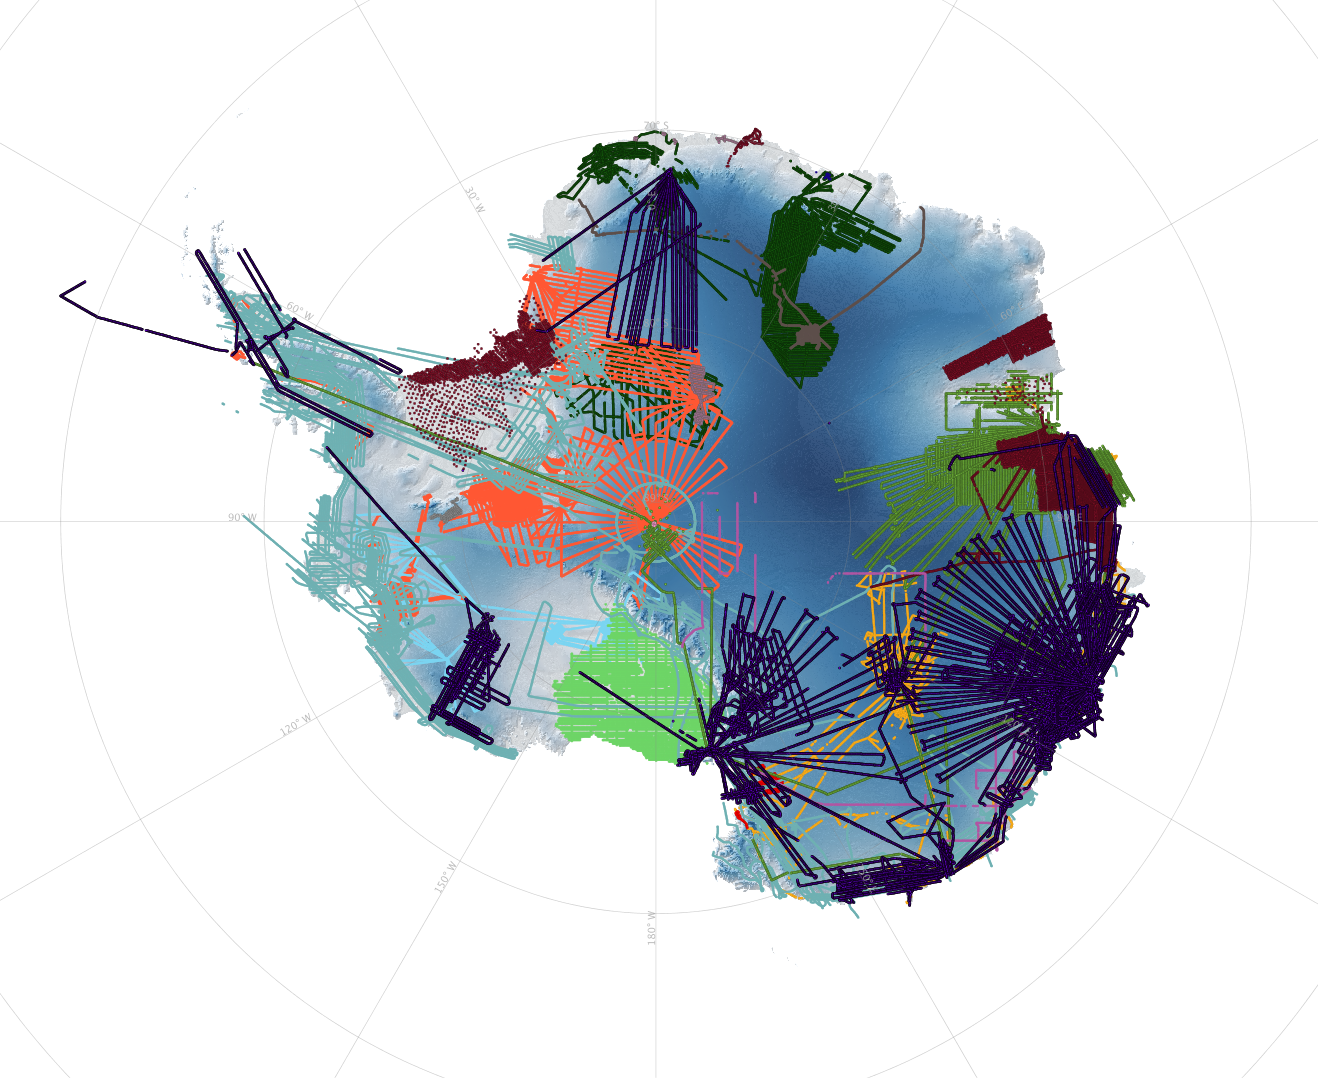
\includegraphics[scale=0.4]{BEDmap3.png}
    \caption{Distribution of BEDmap3 data tracks (Source: bedmap.scar.org).}
\end{figure}

\section*{A case study:\\Critical Factors Influencing Thwaites Glacier's Future Evolution} % [[Castleman_2022]]

Thwaites Glacier in West Antarctica represents one of the most impactful potential contributors to global sea-level rise (SLR), with an estimated contribution of 0.59 meters. The glacier's future evolution is of particular concern because it could trigger a broader collapse of the West Antarctic Ice Sheet. Understanding the factors that control its stability is therefore crucial for accurate sea-level rise projections.

Two primary factors control Thwaites Glacier's evolution\cite{Castleman_2022}: Ocean-driven basal melt rates and bedrock topography. The study reveals that the glacier is highly sensitive to even small changes in bedrock topography within current measurement error bounds, highlighting the critical need for more accurate topographical data.

Current measurement methods rely primarily on ice-penetrating radar, which presents significant challenges. While radar can provide direct measurements along specific tracks, scientists must use interpolation to fill gaps between these tracks. This interpolation introduces statistical uncertainties, particularly in areas where measurements are sparse or rapidly changing. These uncertainties significantly affect our ability to model the glacier's future behavior accurately.

To quantify these uncertainties, Castleman et al.\cite{Castleman_2022} employed two-dimensional discrete wavelet transform (DWT) to systematically analyze and modify bedrock topography data. Their method decomposes a bedrock elevation map $B(x,y)$ into four distinct subarrays: $\mathbf{A}_n$ (low-frequency approximation), and three high-frequency components - $\mathbf{H}_n$ (horizontal), $\mathbf{V}_n$ (vertical), and $\mathbf{D}_n$ (diagonal), where $n$ indicates the decomposition level. 

The researchers selectively amplified the high-frequency components using a multiplier $\alpha > 1$, creating modified arrays $\mathbf{H}'_n = \alpha\mathbf{H}_n$, $\mathbf{V}'_n = \alpha\mathbf{V}_n$, and $\mathbf{D}'_n = \alpha\mathbf{D}_n$. This mathematical approach allowed them to introduce realistic perturbations into bedrock topography models and assess how varying spatial and vertical resolutions affect SLR projections.

One of the study's most significant findings relates to the importance of "pinning points" - bedrock features that can temporarily halt or slow grounding line retreat. While their wavelet-based method could potentially bias results toward more effective pinning points, the study revealed that the location of bedrock features relative to the grounding line and their deviation from mean bed elevation were more significant than feature amplification\cite{Castleman_2022}. Through this analysis, they established crucial requirements for future bedrock measurements: 2 km spatial resolution and $\pm$8 meters vertical accuracy, particularly near the grounding line, to keep SLR uncertainty within $\pm$2 centimeters.

The glacier's vulnerability is further complicated by Marine Ice Sheet Instability (MISI)\cite{Castleman_2022}, a feedback mechanism where warmer ocean temperatures accelerate ice shelf melting and calving. This process is particularly concerning for Thwaites Glacier due to its retrograde bedrock slope\cite{Castleman_2022}, which can accelerate grounding line retreat once initiated.

Ocean-driven basal melt rates present another significant source of uncertainty in ice-sheet model simulations. The challenge stems from the stochastic nature of ocean circulation patterns, temporal variability in ocean forcing, and limitations in current ocean models\cite{Castleman_2022}. These factors make it particularly difficult to predict how the ice sheet will respond to future ocean warming scenarios\cite{Castleman_2022}.

This study underscores the critical importance of accurate bedrock topography measurements for reliable SLR projections. The findings provide clear guidelines for future mapping efforts and highlight the need for focused attention on grounding line regions where bedrock features have the most significant impact on glacier stability.

\section*{Ice Sheet Bed Reconstruction via  Surface Data Inversion} % [[Ockenden_2022]]

Direct observations of ice sheet bed conditions through methods like airborne and ground-penetrating radar or seismic surveying remain sparse, making interpolation and inversion methods necessary for understanding the geophysics. The shape and mechanical properties of the bed significantly influence ice flow behavior, with even small changes in bed conditions potentially causing large variations in predicted ice loss rates. An important observation is that bed features often manifest as subtle signatures in the surface topography above them\cite{Ockenden_2022}.
The relationship between bed and surface characteristics is core to inversion methods that attempt to reconstruct bed properties from surface observations. Unfortunately, these methods cannot paint a complete picture of the ice sheet model. Inversion methods require careful tuning of parameters like the basal friction coefficient, which are not directly observable, so that modelled velocity matches observations. The mathematical framework for these inversions can be achieved via steady-state linear perturbation analysis of shallow-ice-stream equations\cite{Gudmundsson_2008}.

\subsection*{Theoretical Framework}

The foundation of modern bed reconstruction methods lies in the shallow-ice-stream equations (SISEs) of motion (MacAyeal, 1989). These equations describe the relationship between ice flow and bed conditions:
\begin{equation}\partial_{x} (4 h \eta \partial_{x} u + 2 h \eta \partial_y v) + \partial_{y}(h \eta( \partial_{x} v + \partial_{y} u)) - (u/c^{1/m}) = \rho g h ( \partial_{x} (s) \mathrm{cos}(\alpha) - \mathrm{sin}(\alpha))
\end{equation}\\
\begin{equation}\partial_{y} (4 h \eta \partial_{y} v + 2 h \eta \partial_x u) + \partial_{x}(h \eta( \partial_{y} u + \partial_{x} v)) - (v/c^{1/m}) = \rho g h ( \partial_{y} (s) \mathrm{cos}(\alpha)
\end{equation}

where $h$ represents ice thickness, $s$ surface elevation, $(u, v)$ horizontal components of surface velocity, $c$ basal slipperiness, $\eta$ effective ice viscosity, $m$ sliding law parameter, $\rho$ ice density, $\alpha$ mean surface slope in $x$-direction, and $g$ acceleration due to gravity.

\subsection*{Novel Inversion Methodology}

Ockenden et al. develop an innovative inversion method based on steady-state linear perturbation analysis of the SISEs. Their approach introduces perturbations to study how small changes in ice thickness ($h$), surface elevation ($s$), basal topography ($b$), and ice velocity ($u$) affect ice flow. The method assumes:
\begin{enumerate}
\item A linear viscous medium ($n=1$)
\item Non-linear sliding law ($m>0$)
\item Steady-state conditions
\item Spatially constant zero-order solutions
\end{enumerate}

The system is linearized around a reference model $(\bar{h}, \bar{s}, \bar{b}, \bar{u}, \bar{v}, \bar{c})$, leading to first-order momentum balance equations:
\begin{equation}
4 \eta \bar{h} \partial_{xx} \Delta u + 3 \eta \bar{h} \partial_{xy}^{2} \Delta v + \eta \bar{h} \partial_{yy}^{2}\Delta u -\gamma \Delta u  = \rho g \bar{h}\mathrm{cos}(\alpha) \partial_x \Delta s - \rho g \mathrm{sin}(\alpha)\Delta h
\end{equation}\\
\begin{equation}
4 \eta \bar{h} \partial_{yy} \Delta v + 3 \eta \bar{h} \partial_{xy}^{2} \Delta u + \eta \bar{h} \partial_{xx}^{2}\Delta v -\gamma \Delta v  = \rho g \bar{h}\mathrm{cos}(\alpha) \partial_y \Delta s
\end{equation}

\subsection*{Transfer Functions and Implementation}

The methodology employs transfer functions to describe relationships between bed properties and surface characteristics:
$$\begin{bmatrix}
\hat{s} \\
\hat{u} \\
\hat{v}
\end{bmatrix} =\begin{bmatrix}
T_{sb} & T_{sc} \\
T_{ub} & T_{uc} \\
T_{vb} & T_{vc}
\end{bmatrix}
\begin{bmatrix}
\hat{b}\\
\hat{c}
\end{bmatrix}$$
The system is solved using a weighted least-squares approach, minimizing:
\begin{equation}
\Sigma s(s_{\mathrm{obs}} - s_{\mathrm{pred}})^2 + \Sigma u(u_{\mathrm{obs}} - u_{\mathrm{pred}})^2 + \Sigma v(v_{\mathrm{obs}} - v_{\mathrm{pred}})^2
\end{equation}

\subsection*{Application and Limitations}

The method has been successfully implemented using REMA surface elevation data (8m resolution) and NASA ITS\_LIVE velocity data (120m resolution). It performs particularly well in:
\begin{itemize}
\item Areas with moderate topographic gradients in the central trunk of glaciers
\item Features not aligned with ice flow direction
\item Medium-wavelength (5-50km) bedrock features
\end{itemize}
However, the method faces limitations in cases of:
\begin{itemize}
\item Steep topography where shallow-ice-stream approximation breaks down
\item Features aligned with ice flow direction
\item Variable slipperiness parameters
\item Lack of validation data for slipperiness predictions
\end{itemize}
This methodology represents a significant advance in our ability to reconstruct bed conditions using surface data, particularly in regions where direct measurements are sparse or unavailable.




% - [ ] inverse / control method, including BedMachine
% - [ ] 4dvar
% - [ ] monte carlo mass conservation / geostatistics (Mickey Mackie)
% - [ ] EnKF
% - [ ] linear perturbation analysis
% - others?

